\chapter{Development Methodology}

In this project it was chosen to follow an iterative development process. This was chosen because the success criteria for this project is not well defined~\cite{dahlbom1993computers}. The goal of picking which track to play next is a largely subjective decision.

This project being very experimental, following a linear approach could require a large amount of research which has not previously been done, for making descriptive analysis and design documents, before being able to test our theses on how to cope with the problem. Problems which arise later in the process, would then not be handled in an efficient way.

One of the problem with the incremental model compared to the linear waterfall model is that the project can lack structure, since setting milestones with clear goals can be more difficult.

\section{Iterative Design Process}
\label{IterativeDesignProcess}
In the iterative process, the design and implementation is done one step at a time. The development is done in iterations with a new milestone for each iteration. An overview of the process can be seen on \cref{fig:developmentprocess}. These milestones consist of some features which will be analysed, designed, implemented and evaluated, documenting every step in the process. Users will be interviewed in an effort to find new possible problems or requirements, to be taken up for consideration in the following iterations. We will be following these steps through each iteration:

\begin{enumerate}
  \item Gathering data from users and previous iterations
  \item An brief analysis of these data, for declaring new requirements
  \item A comprehensive design phase, researching and choosing concepts in solving these requirements
  \item An effective coding period, implementing the chosen design
  \item Evaluation, consisting mainly of black- and white box testing.
\end{enumerate}

\begin{figure}[hbtp]
  \centering
  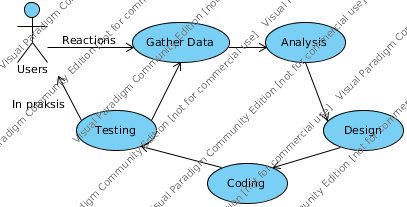
\includegraphics[width=1\linewidth]{Developmentprocess}
  \caption{Overview of the iterative development methodology.}\label{fig:developmentprocess}
\end{figure}

\subsection{Iterations}

Throughout the project the deadlines of the individual iterations will planned according to the project groups semester courses. The first iteration was longer to get the initial prototype working. It is planned for each iteration after that to be of a duration of 14 days each, which adds up to a total of 6 iterations before the project needs to be handed in to the university.
\frnote{ret igennem}

\subsubsection{1\textsuperscript{st} Iteration}

	The project group set out with following milestones for the first iteration:

	Milestones:
	\begin{itemize}
		\item Initial data structure
		\item Be able to vote on a track
		\item Interview bars and pubs about requirements of a music system for their venue.
		\item Communicate a request for a track from one device to another and play it.
	\end{itemize}

	The project group started out with a requirement of being about to count votes on specific tracks to, but we went a little behind schedule due unforeseen details about libspotify, so it was simplified to just communicating a one request.

	In conclusion this was too ambitious while not taking any obstacles in learning how to utilise the Spotify platform, in following iteration planning a margin for learning tools should be accounted for. Not every decision in the design phase was documented in the report, in addition not significant testing were made.
	\frnote{Vise mere frem af hvad vi opnåede }

\subsubsection{2\textsuperscript{nd} Iteration}

	On behalf of the experience made in previous iteration, about being to ambitious in meeting all milestones at deadline, another approach is introduced, by classifying each milestone under what \enquote{Must} and what \enquote{Should} be done this iteration. An emphasise will be put on documentation and testing on milestones of 2nd iteration:

	Must:
	\begin{itemize}
		\item Interview everyday users about requirements for music system.
		\item Do a section on concepts in the system
	\end{itemize}

	Should:
	\begin{itemize}
		\item Document previously taken decisions
		\item Describe architecture
		\item Do a comprehensive testing section
		\item Make a democratic handling on the backend
	\end{itemize}

\subsubsection{3\textsuperscript{rd} Iteration}

  The way of making goals for the iterations changed yet again, to make goals for each part of the report, these parts also match the development cycle. This means we could conclude on each step of the cycle and which showed to be beneficial, in that we could track the progression of each concept included in the project through the development cycle from \enquote{Data Collection} to \enquote{Testing}.

  Gather Data:
  \begin{itemize}
    \item Interview and showcase demo for collaboration partner "Fabrikken".
  \end{itemize}

  Analysis:
  \begin{itemize}
    \item Document interview
    \item Extract requirements
    \item Revisit classes to account for restrictions.
  \end{itemize}

  Design:
  \begin{itemize}
    \item Restriction design
    \item Revisit Architecture
  \end{itemize}

  Implementation:
  \begin{itemize}
    \item Implement restriction design
    \item Document patterns used for this
  \end{itemize}

  Testing:
  \begin{itemize}
    \item Test restrictions works as intented by unit testing.
    \item Test restrictions in context of users.
  \end{itemize}

\subsubsection{4\textsuperscript{th} Iteration}

  We finally kept the method of making goals for the iterations, we followed the same process as previous iteration, only with an presentation interface this time.
